\section{QoI Model}
\label{sec:qoi_model}

We want to look at a number of information attributes that all impact the Quality of Information.  Specifically, we want to study the following:

\begin{itemize}
  \item Precision
  \item Accuracy
  \item Completeness
  \item Age
  \item Timeliness
\end{itemize}

The first two attributes, precision and accuracy, are determined by inherent qualities of the data with respect to the goal of the application that it supports.  One example would be a facial recognition application.  

Completeness is a metric that is mostly evaluated within the context of the application's goals and the whole of information being used to support it.  For example, if a surveillance application seeks to obtain at least one image of every block in a desired area of a city, then the completeness of a set of images is defined by how many of the blocks are actually visible in the collected images.  Further examples are explored in depth in the DCOSS submission.

Age and timeliness are both time-based attributes that each contribute to QoI in different manners.  Age describes how long ago the information was generated.  The importance of age is highly dependent upon the context in which the information is being used.  Timeliness of information describes the time between when it is requested and when it is obtained.  

Again, images are good examples for these two metrics.  Let's say a known criminal is suspected to have been spotted, but an image of the criminal is needed to compare to the suspected individual.  If the application is facial recognition software, then an image that is up to several years old may be acceptable since face structure does not change much, but if a user is attempting to make the identification, then a more recent photo may be necessary to account for changes like change in weight or hairstyle.  If we assume that the criminal should be apprehended, then the timeliness in receiving the image with which to identify the suspect is important because it is only useful while the suspect is under surveillance.  

Now, we want to examine the differences in how each of these QoI attributes is impacted by various effects, such as time, capacity, and load.  Furthermore, we want to capture how these impacts occur in computer memories vs. human memories.

\subsection{Precision}

\begin{figure}
\begin{centering}
    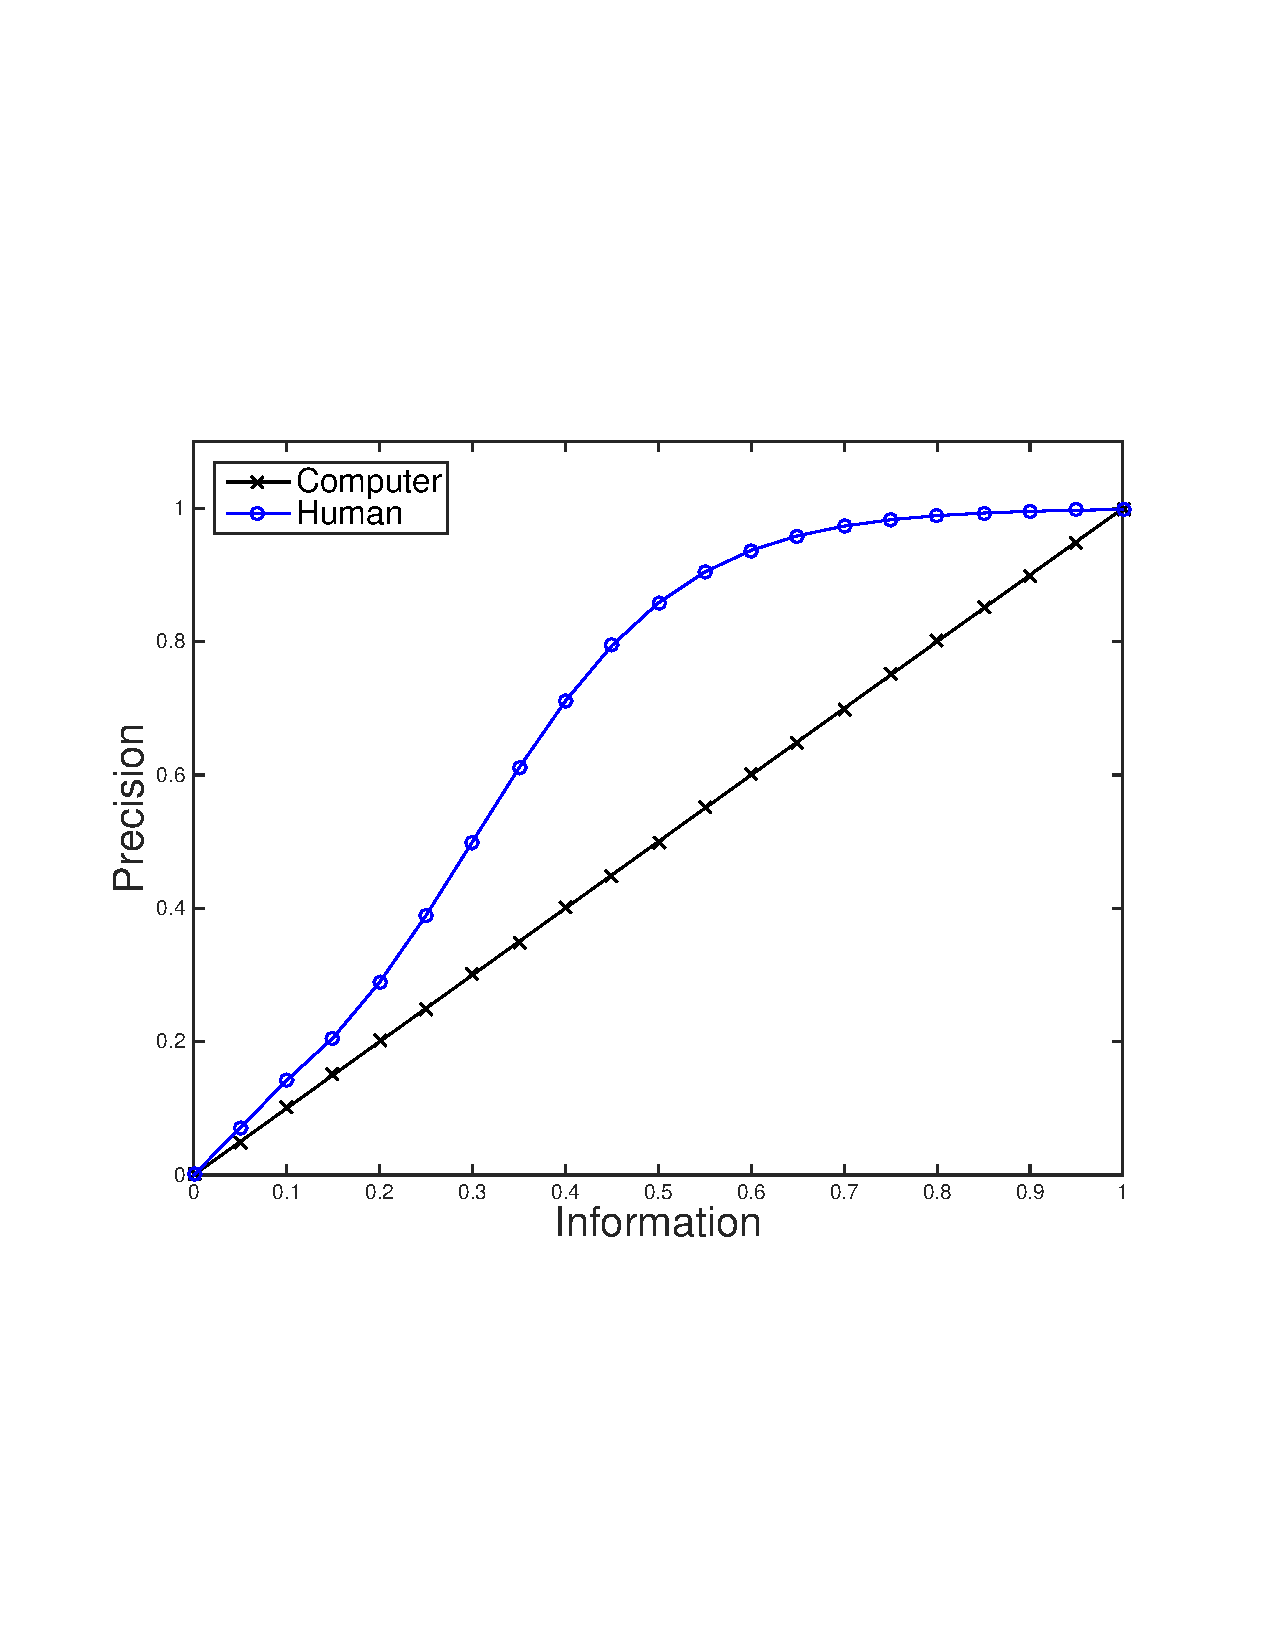
\includegraphics[clip=true, trim = 15mm 65mm 25mm 70mm, scale=0.40]{figures/example_qoi_trends/prec_vs_info_hvc_1.pdf}
    \caption{Precision with more Infomation in Computers vs. Humans }
    \label{fig:prec_vs_info_hvc}
\end{centering}
\end{figure}

When considering \emph{precision}, perhaps we can look at the following question:  How much detail do we have describing the situation of interest? 

When storing information in computers, the amount of precision that can be retrieved is simply equal to the amount of information that is stored.  This process is unitary.  

Human memory is commonly perceived to be a dual-storage process, in which people store both \emph{verbatim} and \emph{gist} representations of an event.  

In a scenario with context, humans gain an advantage over computers because of their ability to contextualize new information with previous knowledge and draw conclusions, effectively adding more information.  Figure \ref{fig:prec_vs_info_hvc} represents this phenomenon showing that as more information is collected, a human is able to provide more detail, increasing the precision above the baseline of the linear accumulation that occurs with a computer.  
 

%For example, if we ask for a weather forecast, an answer of $25$ degrees Fahrenheit is a more precise answer than ``It's cold."  

\begin{figure}
\begin{centering}
    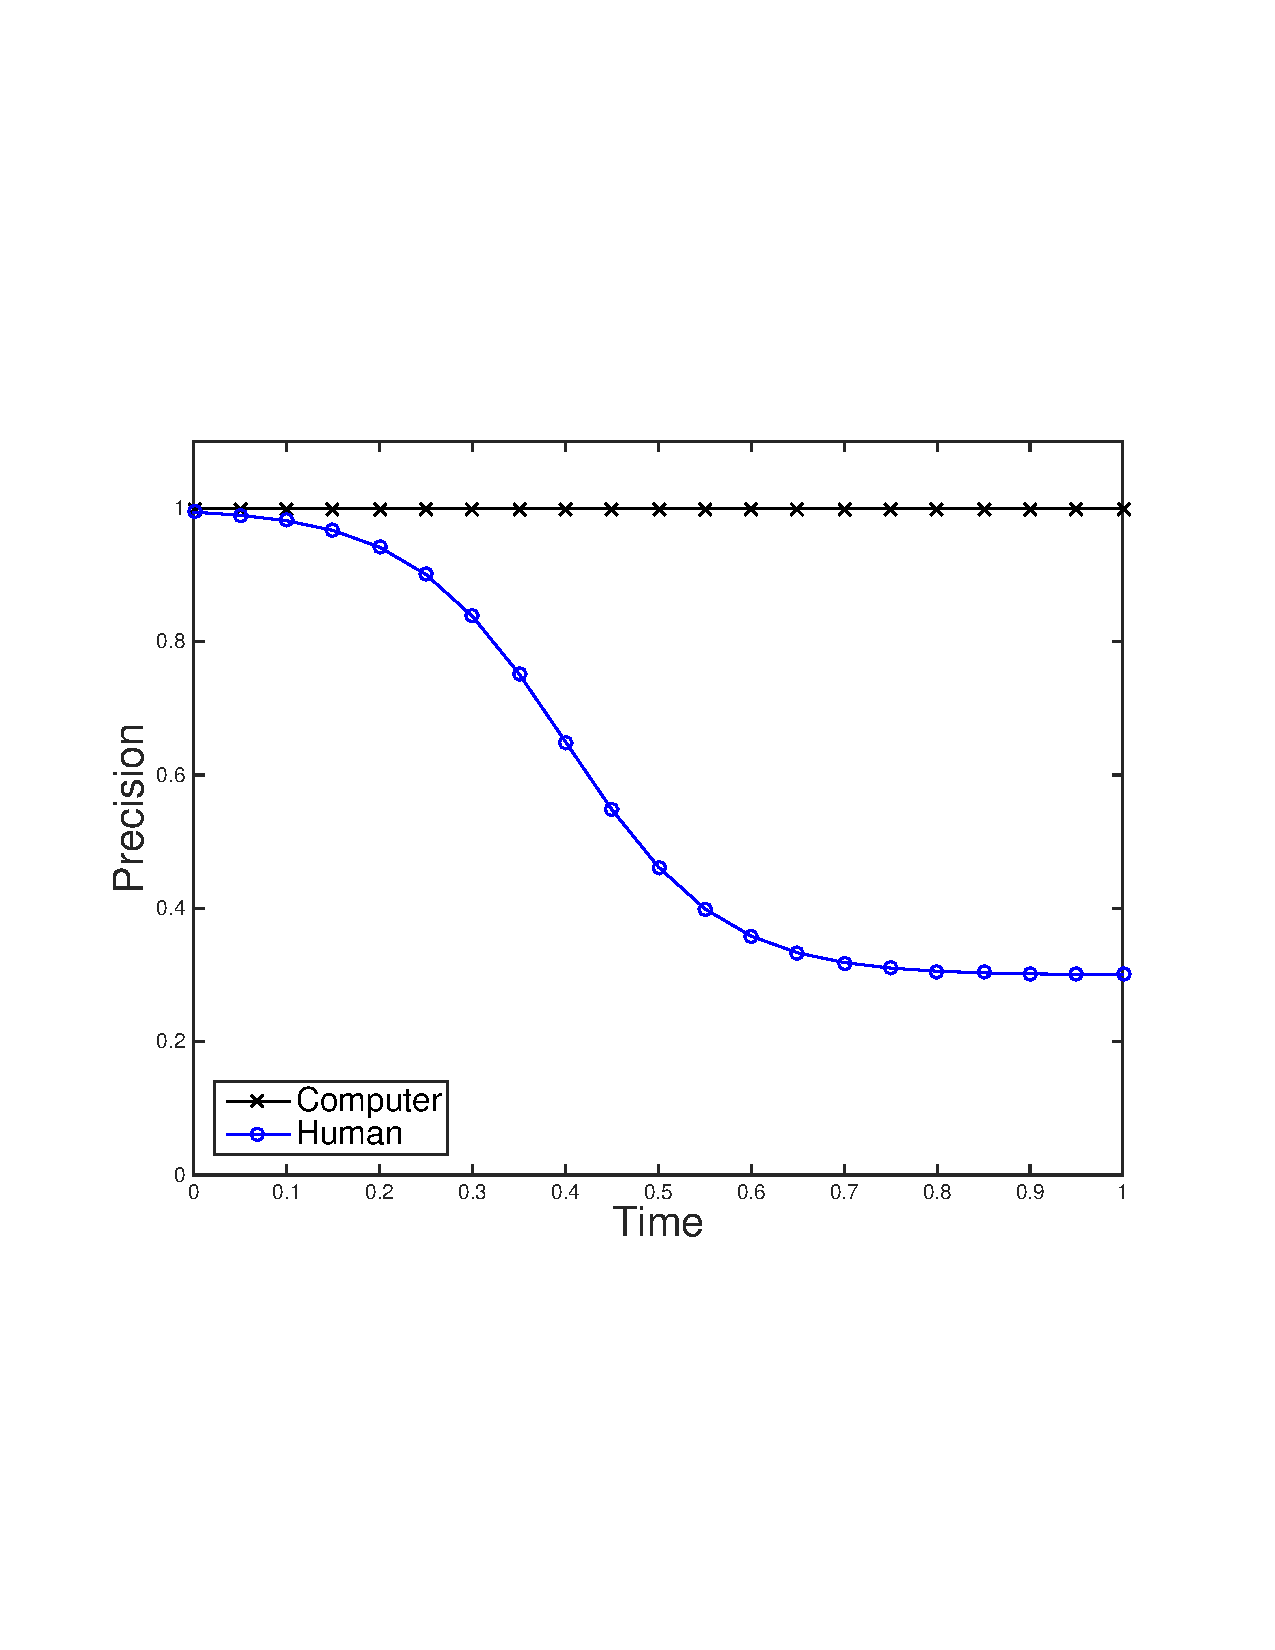
\includegraphics[clip=true, trim = 15mm 65mm 25mm 70mm, scale=0.40]{figures/example_qoi_trends/prec_vs_time_hvc_1.pdf}
    \caption{Precision as Time Passes in Computers vs. Humans }
    \label{fig:prec_vs_time_hvc}
\end{centering}
\end{figure}

As time passes, though, humans will forget or merge details, whereas a computer memory is unchanging.  Therefore, as shown in Figure \ref{fig:prec_vs_time_hvc}, the level of detail in human memory degrades over time.  Of course, some general information remains, so the precision levels off at some non-zero minimum.

\subsection{Accuracy}

We loosely define \emph{accuracy} as how close a stored data value, $d$, is to the corresponding real-world value of $d'$, as in \cite{batini2009methodologies}.  If the value is objective, like the temperature at a location, measuring the accuracy of a value is straightforward. 

\subsubsection{General}
\begin{figure}
\begin{centering}
    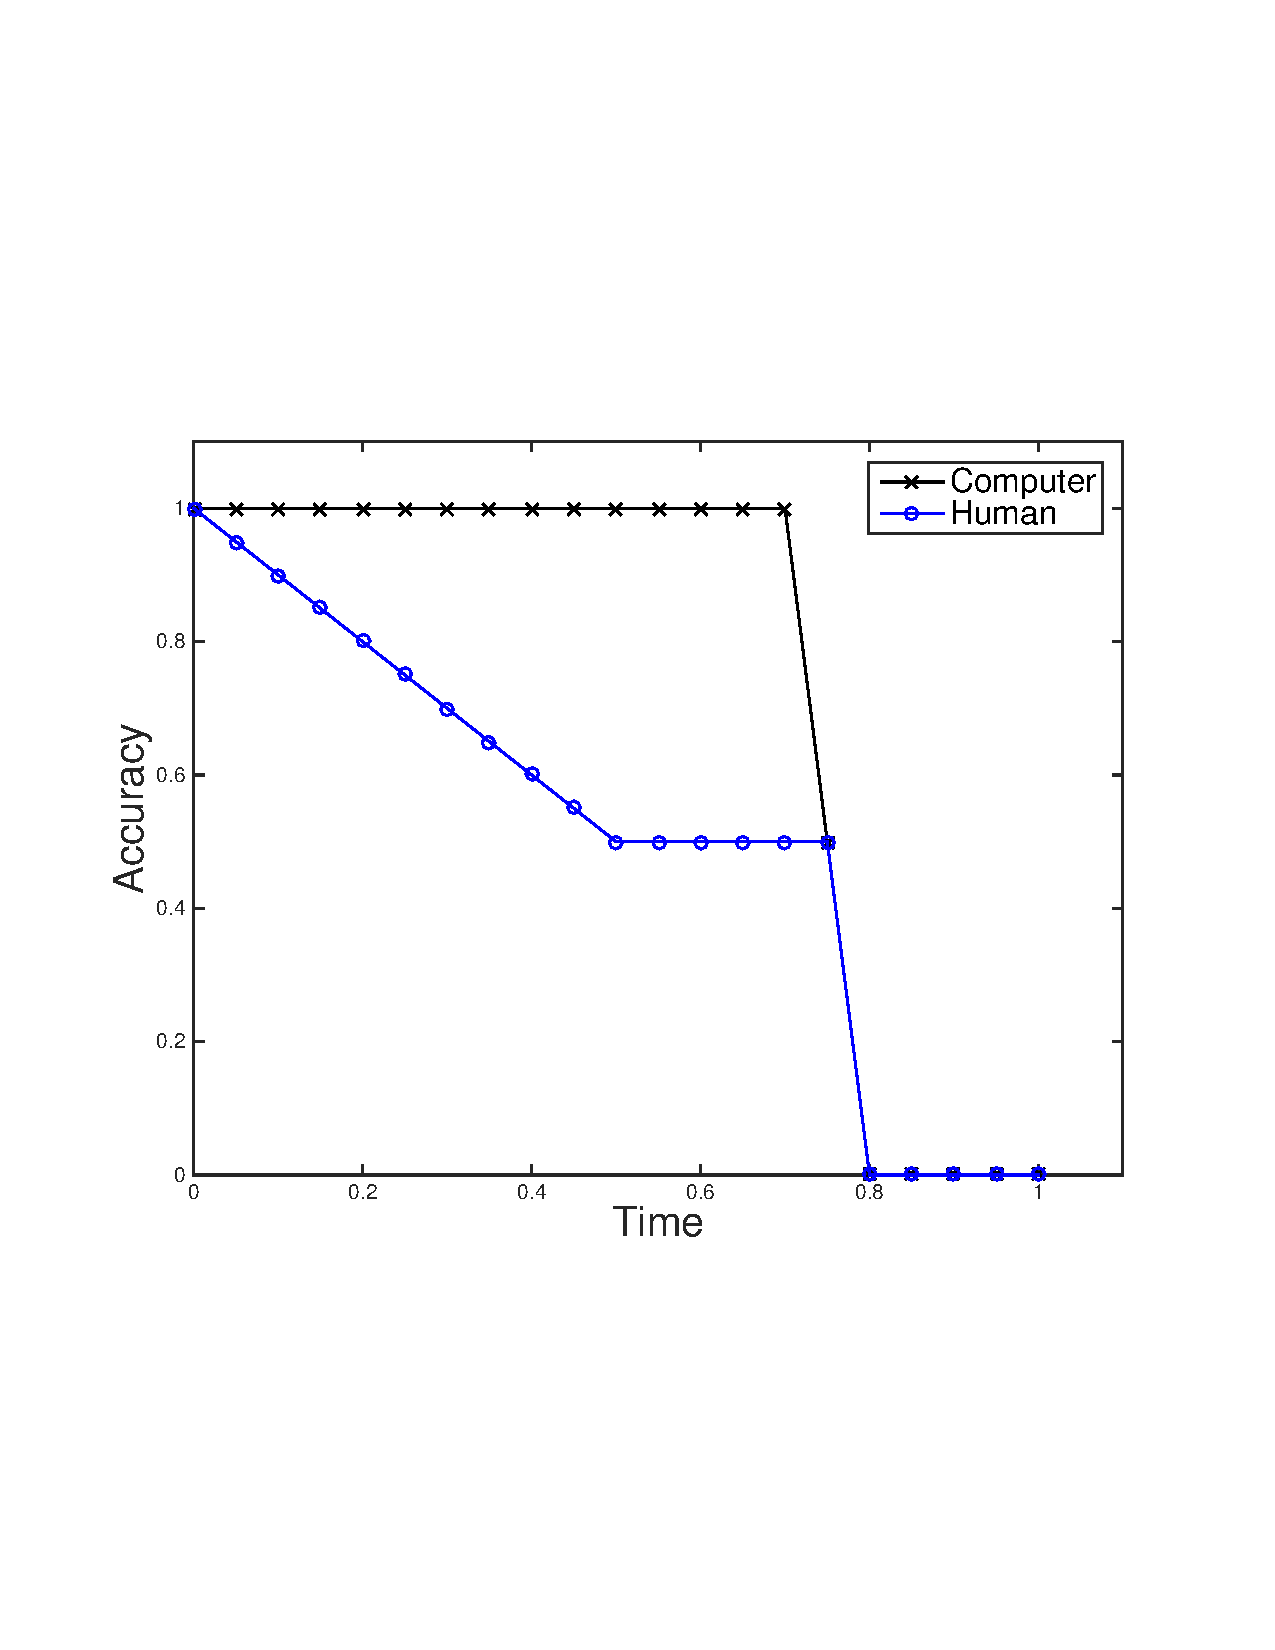
\includegraphics[clip=true, trim = 15mm 65mm 25mm 70mm, scale=0.40]{figures/example_qoi_trends/accuracy_hvc_2.pdf}
    \caption{Loss of Accuracy over Time in Computers vs. Humans }
    \label{fig:acc_vs_time_hvc_gen}
\end{centering}
\end{figure}

We propose a general model of how accuracy is affected by the time for which things are stored.  Since computer memories do not modify any data contents, the accuracy of the data is only affected by its invalidation due to the source creating new data that invalidates the data in the cache.  At this point, the accuracy goes to zero.  In a human memory, the same timeout occurs eliminating the accuracy of the data at the point in which new information is created, but not yet achieved.  The time period before this timeout, however, is different for a human memory because human memories are lossy over time.  Therefore, a human begins to lose accuracy of obtained information almost immediately.  This loss continues for a period of time, until a threshold of a minimum accuracy that is retained.  This minimum accuracy is retained until the information is past the timeout for it to retain any intrinsic accuracy at all.  Examples of these two trends are shown in Figure \ref{fig:acc_vs_time_hvc_gen}.

\subsubsection{Facial Recognition}

For most applications that of interest here, like facial recognition for example, accuracy may be best defined as a confidence level or the likelihood of achieving a correct identification with the supplied information.  

\begin{figure}
\begin{centering}
    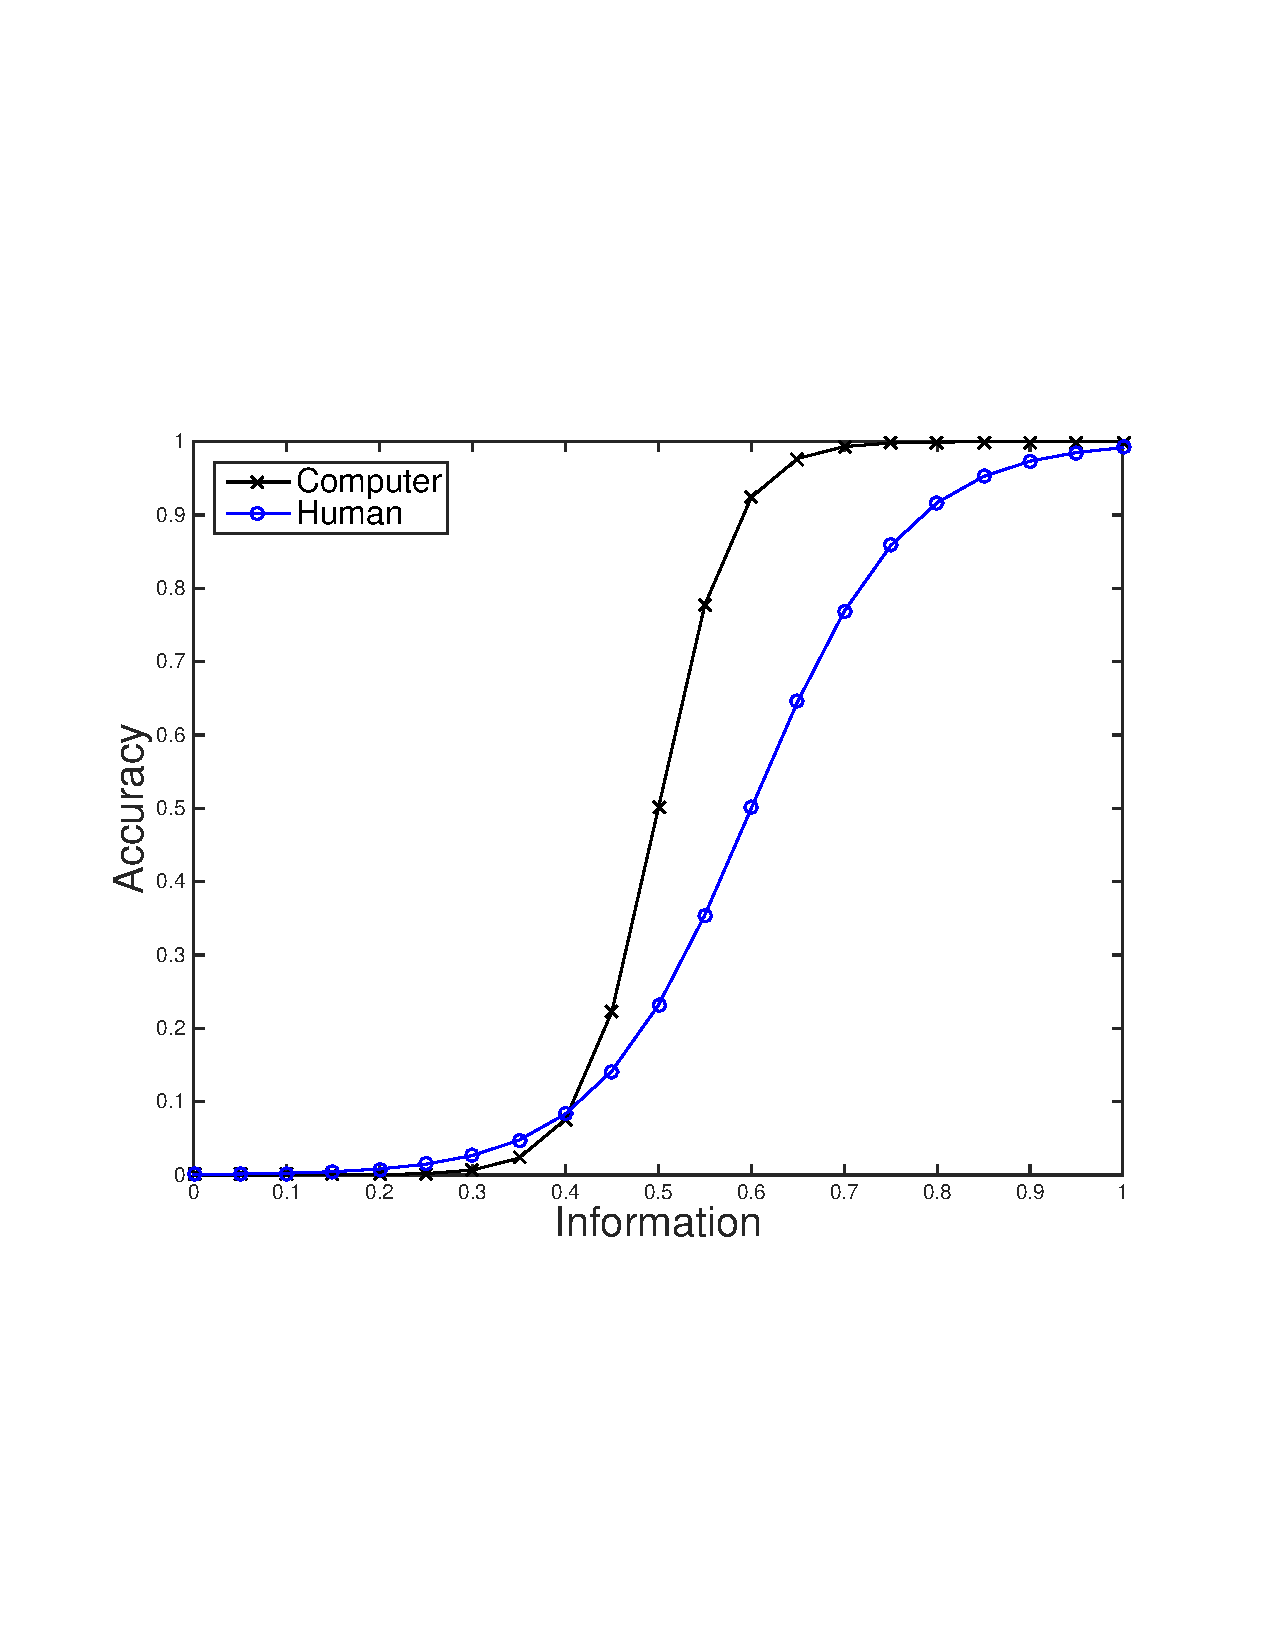
\includegraphics[clip=true, trim = 15mm 65mm 25mm 70mm, scale=0.40]{figures/example_qoi_trends/acc_vs_info_hvc_FR.pdf}
    \caption{Accuracy of Facial Recognition with more Infomation in Computers vs. Humans }
    \label{fig:acc_vs_info_hvc_FR}
\end{centering}
\end{figure}

Using this application as an example, we can compare the effectiveness with increasing information.  As shown in \cite{qoi_aware_mobile_apps}, image processing techniques can withstand a certain level of compression while remaining almost perfectly accurate.  Once a certain compression threshold is reached, though, the ability of the facial recognition application to correctly classify an image drops off dramatically.  We propose that the same effect would occur in humans, but that a human's threshold for compression in successful identification is lower, thus requiring them to receive more information, i.e. higher resolution files, to achieve a high likelihood of success.  These trends are shown in Figure \ref{fig:acc_vs_info_hvc_FR}.

\begin{figure}
\begin{centering}
    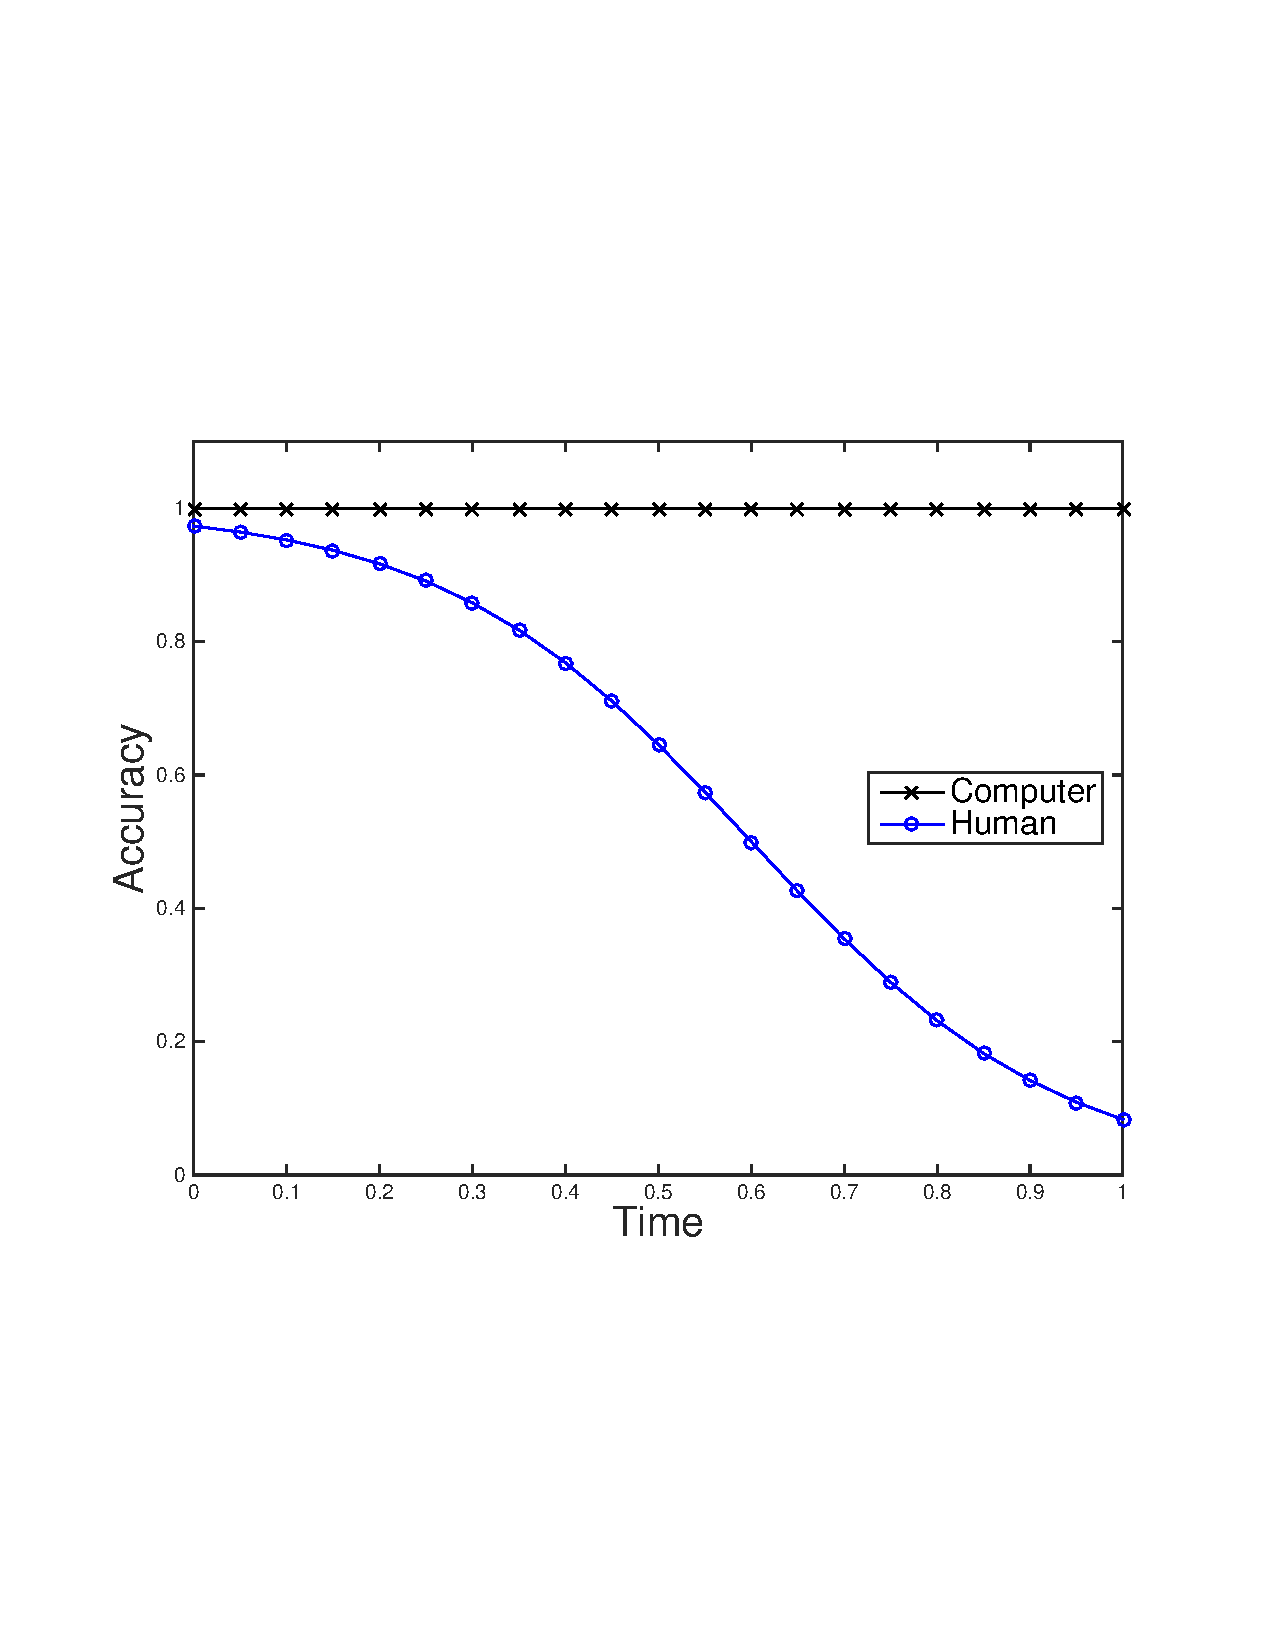
\includegraphics[clip=true, trim = 15mm 65mm 25mm 70mm, scale=0.40]{figures/example_qoi_trends/acc_vs_time_hvc_FR.pdf}
    \caption{Loss of Accuracy in Facial Recognition over Time in Computers vs. Humans }
    \label{fig:acc_vs_time_hvc_FR}
\end{centering}
\end{figure}

\subsection{Completeness}

\begin{figure}
\begin{centering}
    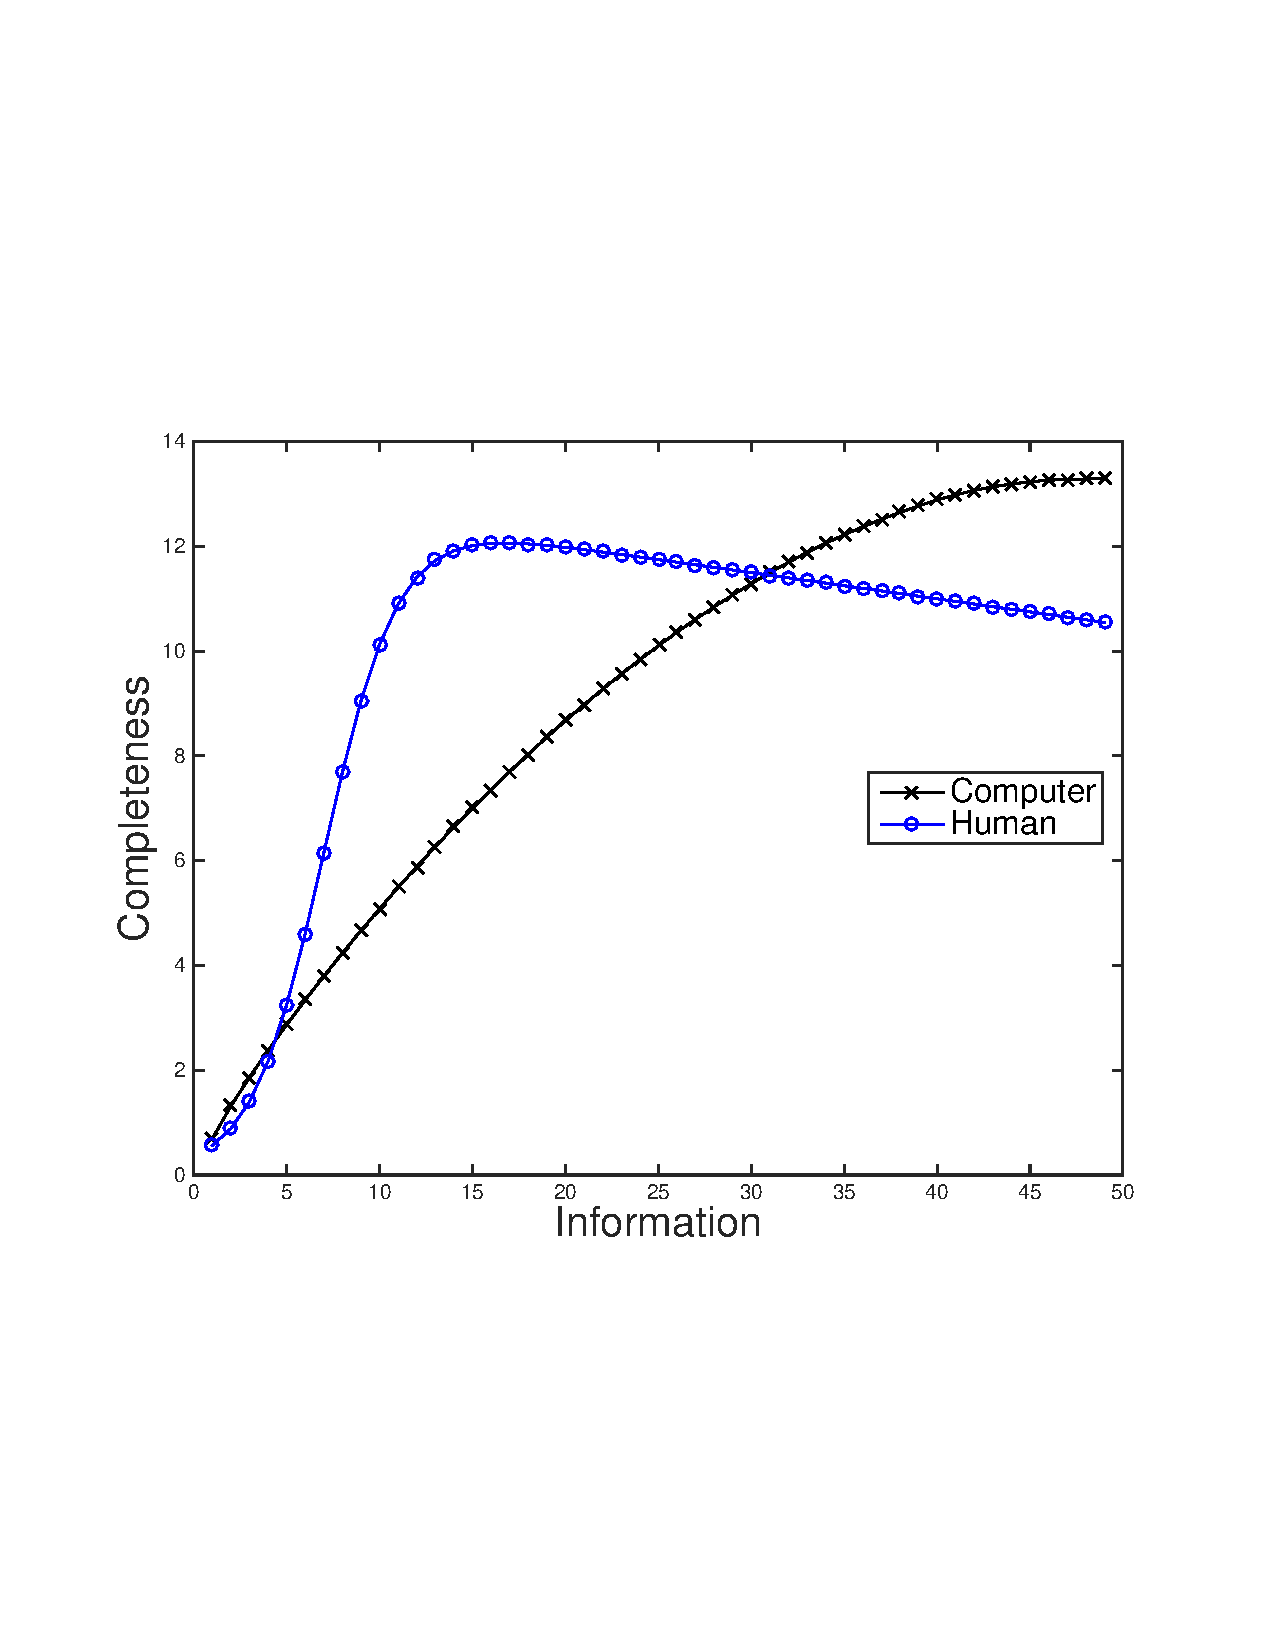
\includegraphics[clip=true, trim = 15mm 65mm 25mm 70mm, scale=0.40]{figures/example_qoi_trends/completeness_vs_info_hvc.pdf}
    \caption{Information Overload in Computers vs. Humans }
    \label{fig:comp_vs_info_hvc}
\end{centering}
\end{figure}

\begin{figure}
\begin{centering}
    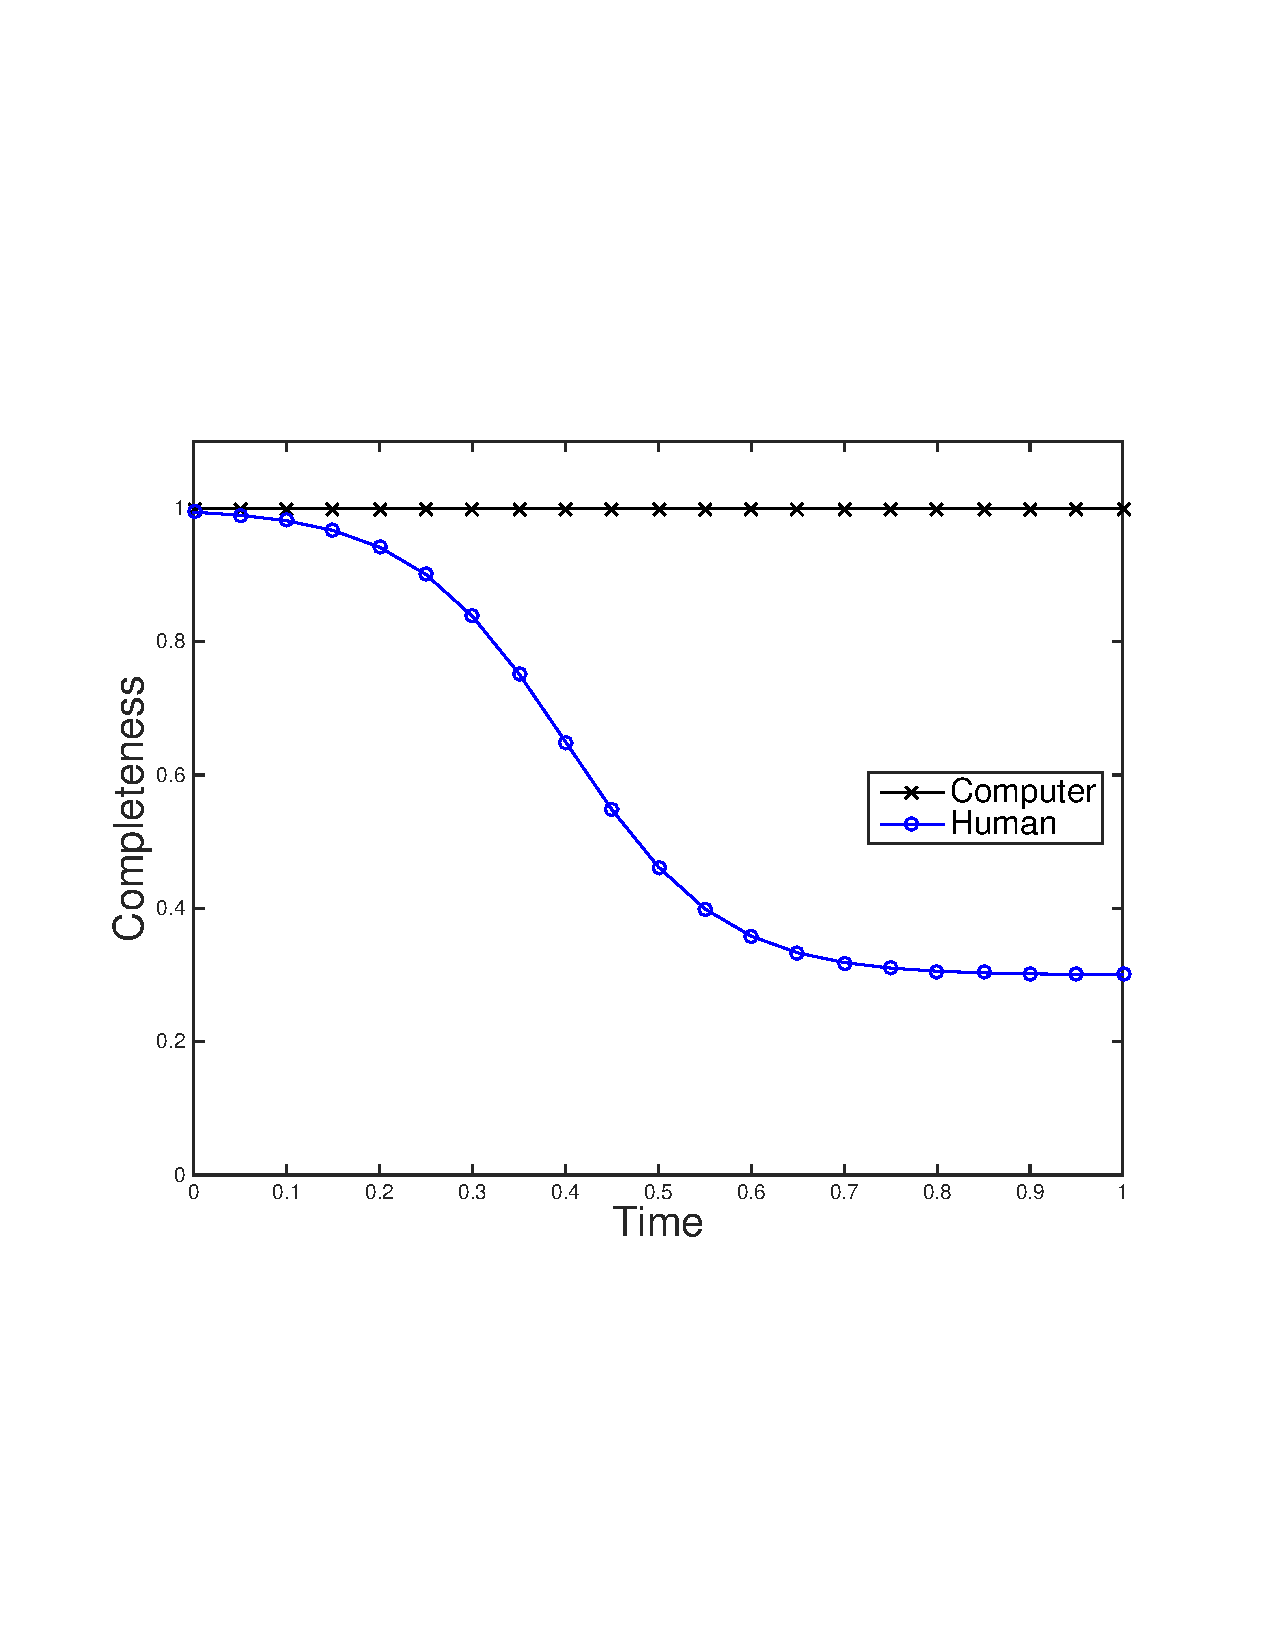
\includegraphics[clip=true, trim = 15mm 65mm 25mm 70mm, scale=0.40]{figures/example_qoi_trends/completeness_vs_time_hvc.pdf}
    \caption{ Loss of Completeness in Human Memory over Time }
    \label{fig:comp_vs_time_hvc}
\end{centering}
\end{figure}

As in the most recent work (DCOSS 2015 submission), we showed a diminishing returns on completeness as information load is increased.  In humans, completeness is quickly gained as information is first received, because they are efficient in pulling important details and obtaining the gist of what is important.  Of course, humans have a finite capacity of completeness of information, and experience an overloading after a certain amount of information is received that is not entirely relevant.  These trends are shown in Figure \ref{fig:comp_vs_info_hvc}.

Figure \ref{fig:comp_vs_time_hvc} captures the mutation of completeness of information over time.  In a computer, completeness does not change with time, since data is immutable.  Again, in a human memory, loss occurs over time, but not completely.  

\subsection{Age}
The age of information simply refers to how long ago the information was generated.  This metric would be no different in human memory vs. computer memory.  

\subsection{Timeliness}
Timeliness refers to the delay incurred between a request being generated and the requested information being delivered to the requesting party.  Note that this metric is distinct from the age of the information.  For example, an image in a database may have been taken five minutes ago or last week.  That detail describes the age of the information.  If a user connects to the database, and the download time is $30$ seconds, then the timeliness of the delivered image is $30$ seconds.  

We expect that timeliness will be dominated by the network over which information is transmitted, not memory access time, so we do not outline a difference between human and computer nodes here.  (Are there circumstances in which humans require a non-trivial amount of time to recall information that we should consider here?)
